\subsection{Winston cone refurbishment}

Winston cones (WC) are used to collect light onto the PMTs. In the LTCC there are three kind of WCs:

\begin{enumerate}

\item Small
	\begin{enumerate}
		\item Height: 18 cm
		\item Radius at the top: 20 cm
		\item Radius at the bottom: 11 cm
		\item Material: 0.25 cm thick copper (electro-formed)
	\end{enumerate}

	\item Medium
	\begin{enumerate}
		\item Height: 22 cm
		\item Radius at the top: 20 cm
		\item Radius at the bottom: 11 cm
		\item Material: 0.5 cm thick plastic (vacuum pressed)
	\end{enumerate}

	\item Large
	\begin{enumerate}
		\item Height: 30 cm
		\item Radius at the top: 22 cm
		\item Radius at the bottom: 11 cm
		\item Material: 0.25 cm thick copper (electro-formed)
	\end{enumerate}
\end{enumerate}

\begin{figure}
	\centering
	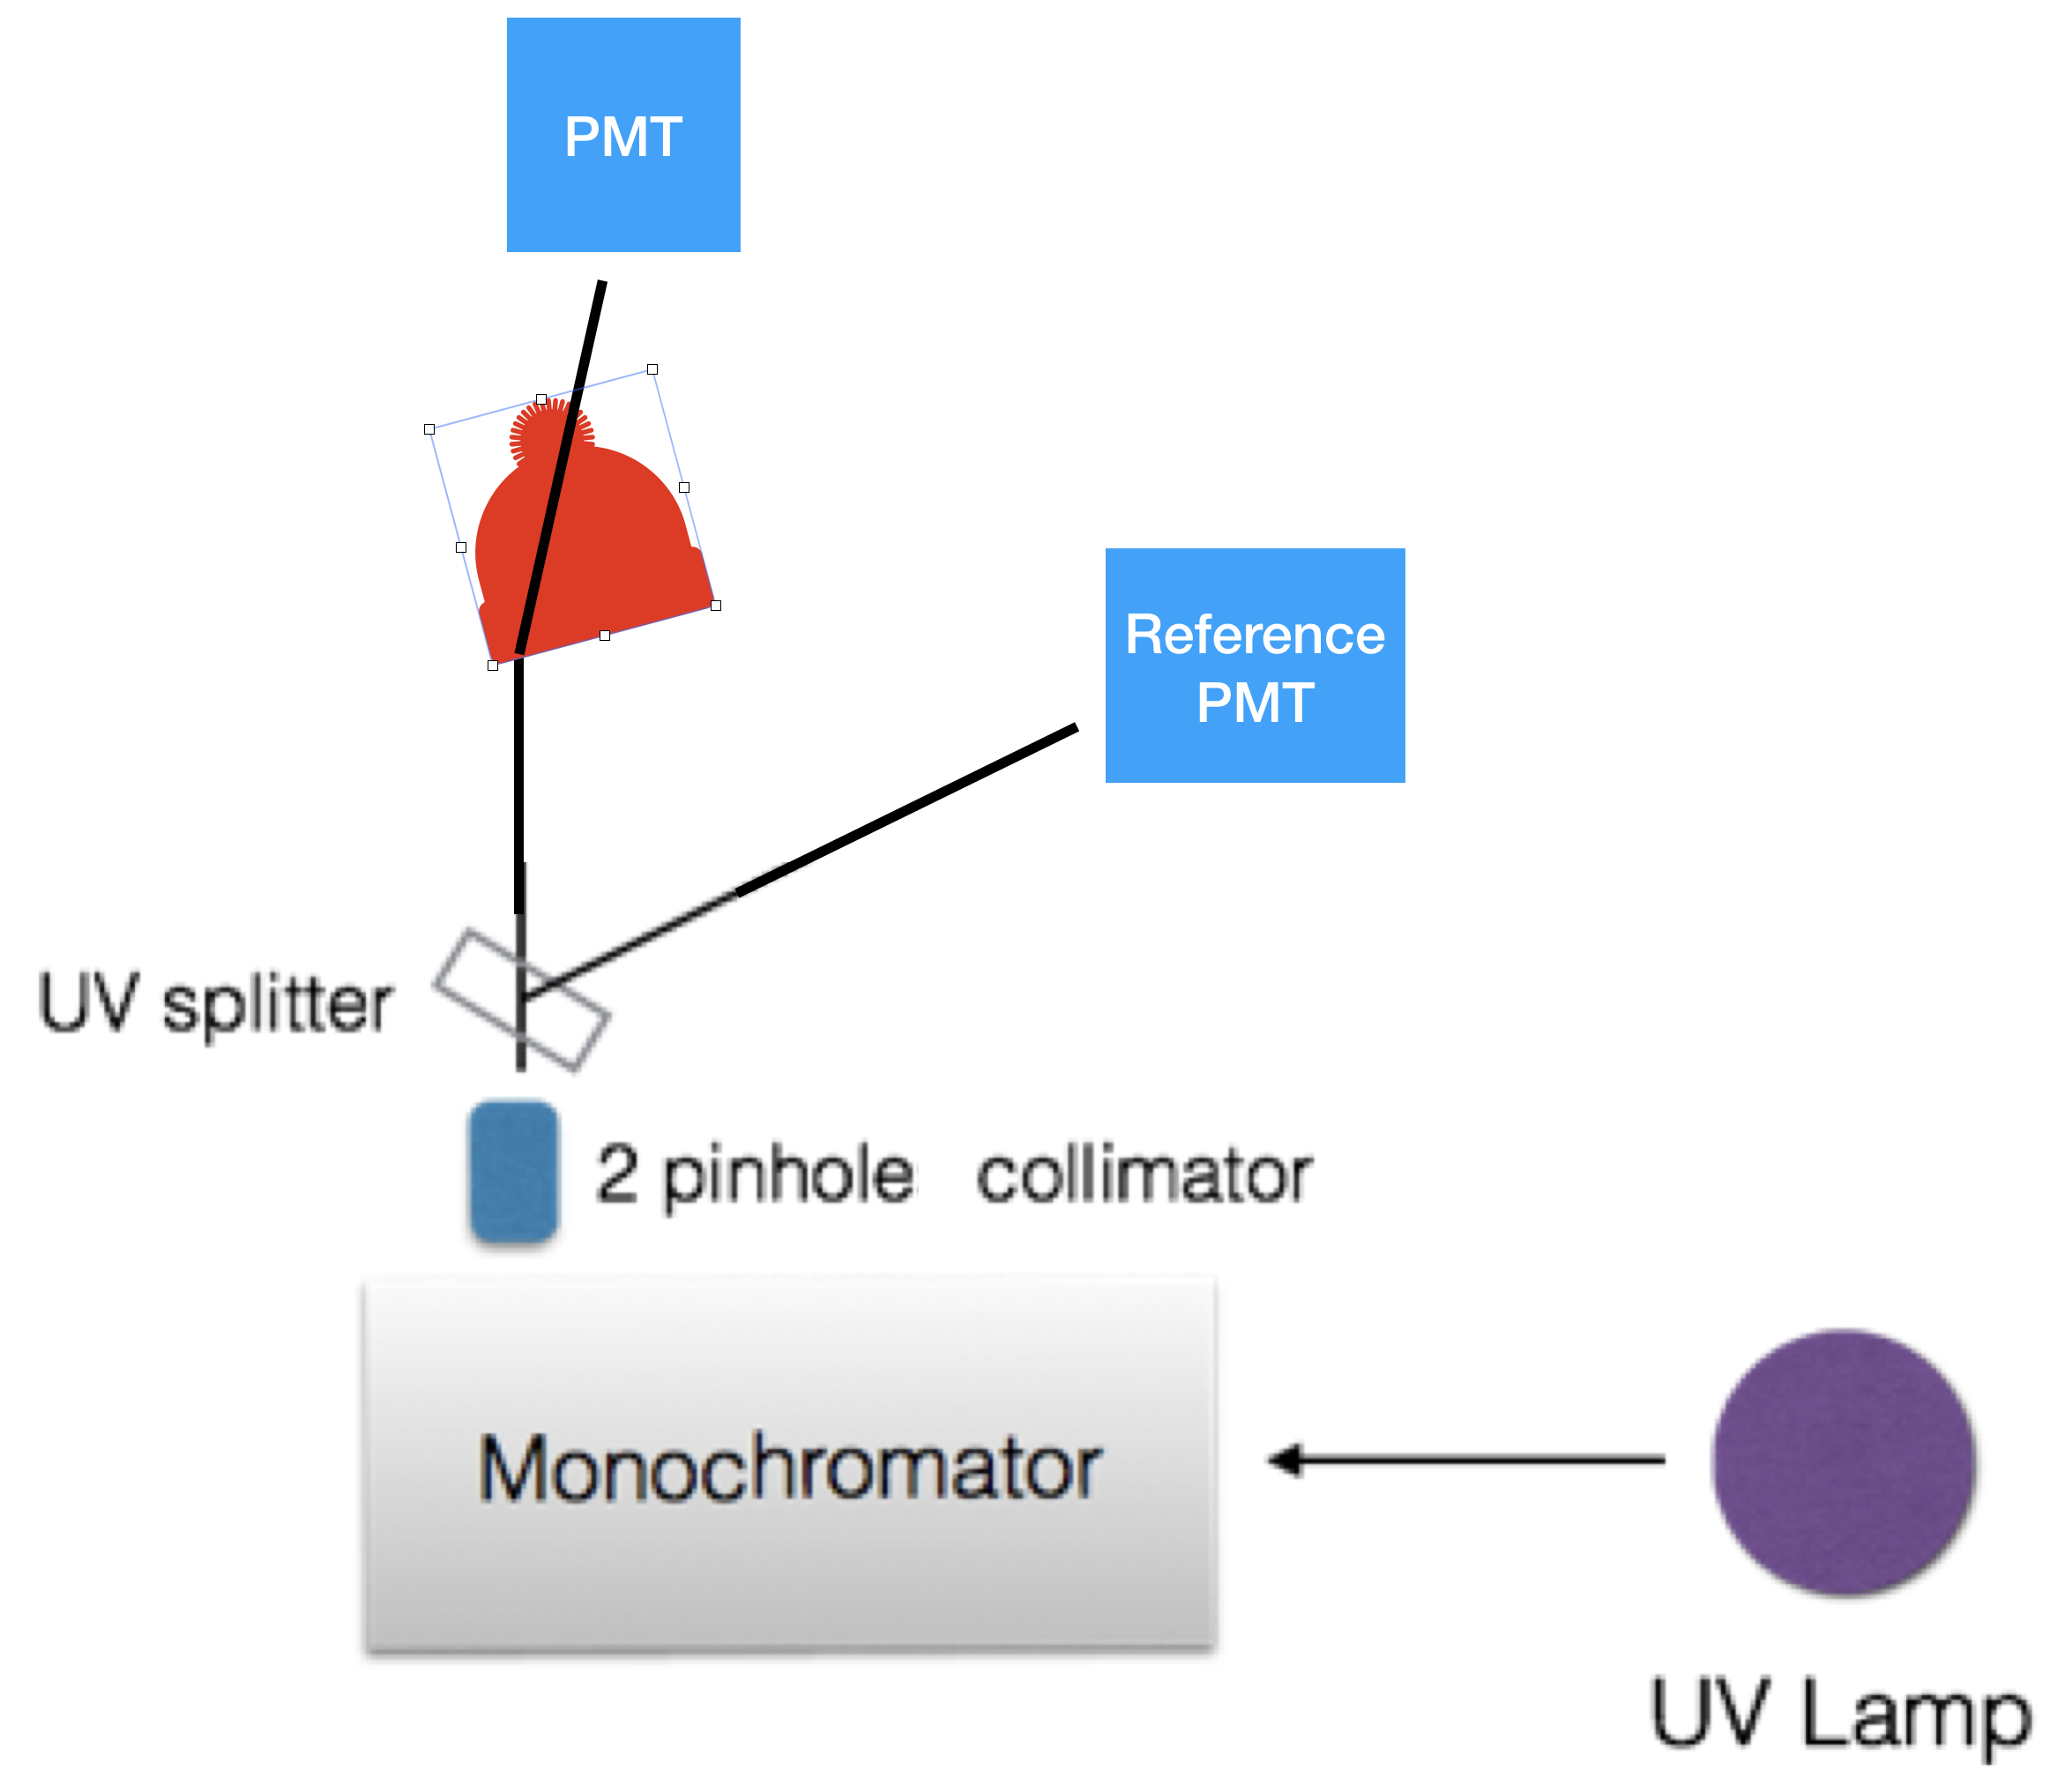
\includegraphics[width=0.95\columnwidth,keepaspectratio]{img/wcSetup.png}
	\caption{Setup to measure the WC reflectivity. The wavelength of light from a deuterium lamp was measured using a monochromator and split in two
            light beams, each with calibrated intensity. One of the light beams impinged on the WC at a typical angle of 12 degrees,
            while the other was directed at the reference PMT. The reflectivity was measured in different spots for a sample of WCs.  The results proved
            to be independent on the spot. }
	\label{fig:wcSetup}
\end{figure}

The reflectivity of the WC showed the same degradation as the mirrors. However, due to their shape, re-coating of the WC is more costly than the mirrors and the budget allowed
refurbishing of only 160 out of 216 total WCs.
A setup on an optical bench to measure the reflectivity for all the cones at wavelengths between 200 and 400 nm was designed to accept incident
shallow angles of 10-15 degrees (typical incidence angle based on simulation studies), see \F{wcSetup}. A typical reflectivity of a poor WC is shown in \F{wcStatusBefore} (top).
All 216 WC were measured, and the results are shown in \F{wcStatusBefore} (top). A sample of the WCs This allowed cataloging of the quality of the WC to select the worst ones to refurbish,
see \F{wcStatusBefore} (bottom).
The cones were put in a vacuum chamber and AlMgF$_2$ was deposited on top of the existing coating. The typical reflectivity of WC after coating is shown in \F{wcStatusAfter} (top).
About 30 cones needed the additional treatment of removing the existing aluminum coating to improve the new AlMgF$_2$ deposition. Even then, about half of these cones did not show improvements.
The results of the WCs refurbishment are summarized in \F{wcStatusAfter} (bottom).


\begin{figure}[h]
	\centering
	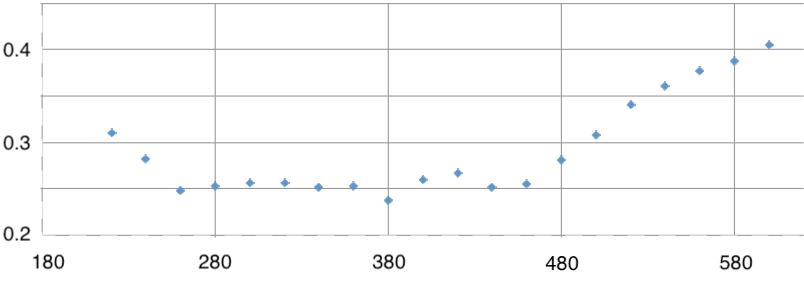
\includegraphics[width=0.95\columnwidth,keepaspectratio]{img/winstoConeSample2Reflectivity.png}
	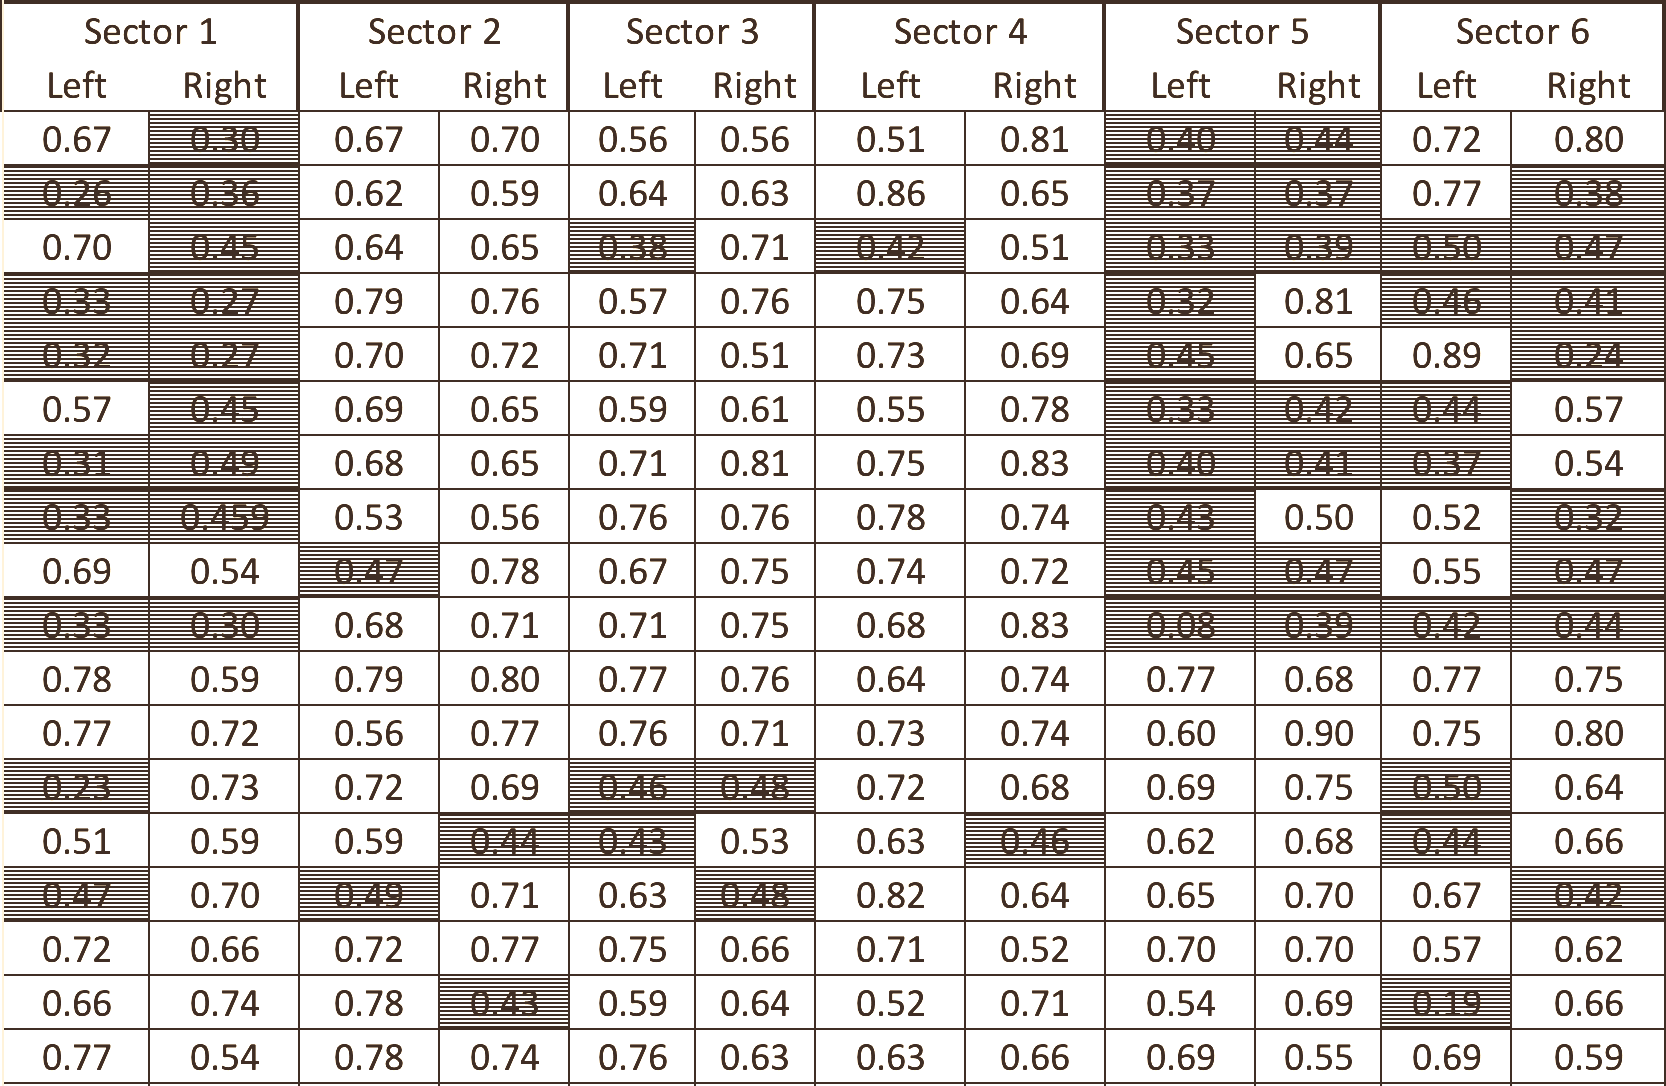
\includegraphics[width=0.95\columnwidth,keepaspectratio]{img/wcStatusBefore.png}
	\caption{Top: typical reflectivity of a``very poor'' WC. The reflectivity is below 30\% for most wavelengths between 200 and 400 nm. The reflectivity proved to be independent on the
				particular spot on the WC surfaces.
            Bottom: the average reflectivity $r$ between 200 and 400 nm for all WCs. Legend: grey: ``very poor'' ($r < 30\%$);
            red: ``poor'' ($30\% < r < 50\%$); yellow: ``average quality'' ($50\% < r < 70\%$); green: ``good'' ($70\% < r < 80\%$); cyan: ``excellent'' ( $r > 80\%$); }
	\label{fig:wcStatusBefore}
\end{figure}


\begin{figure}[h]
	\centering
	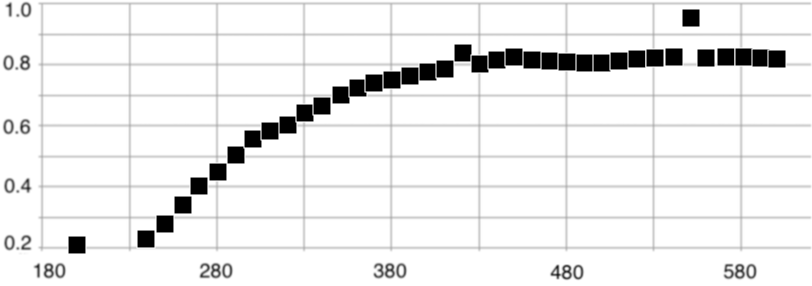
\includegraphics[width=0.95\columnwidth,keepaspectratio]{img/winstoConeSample1Reflectivity.png}
	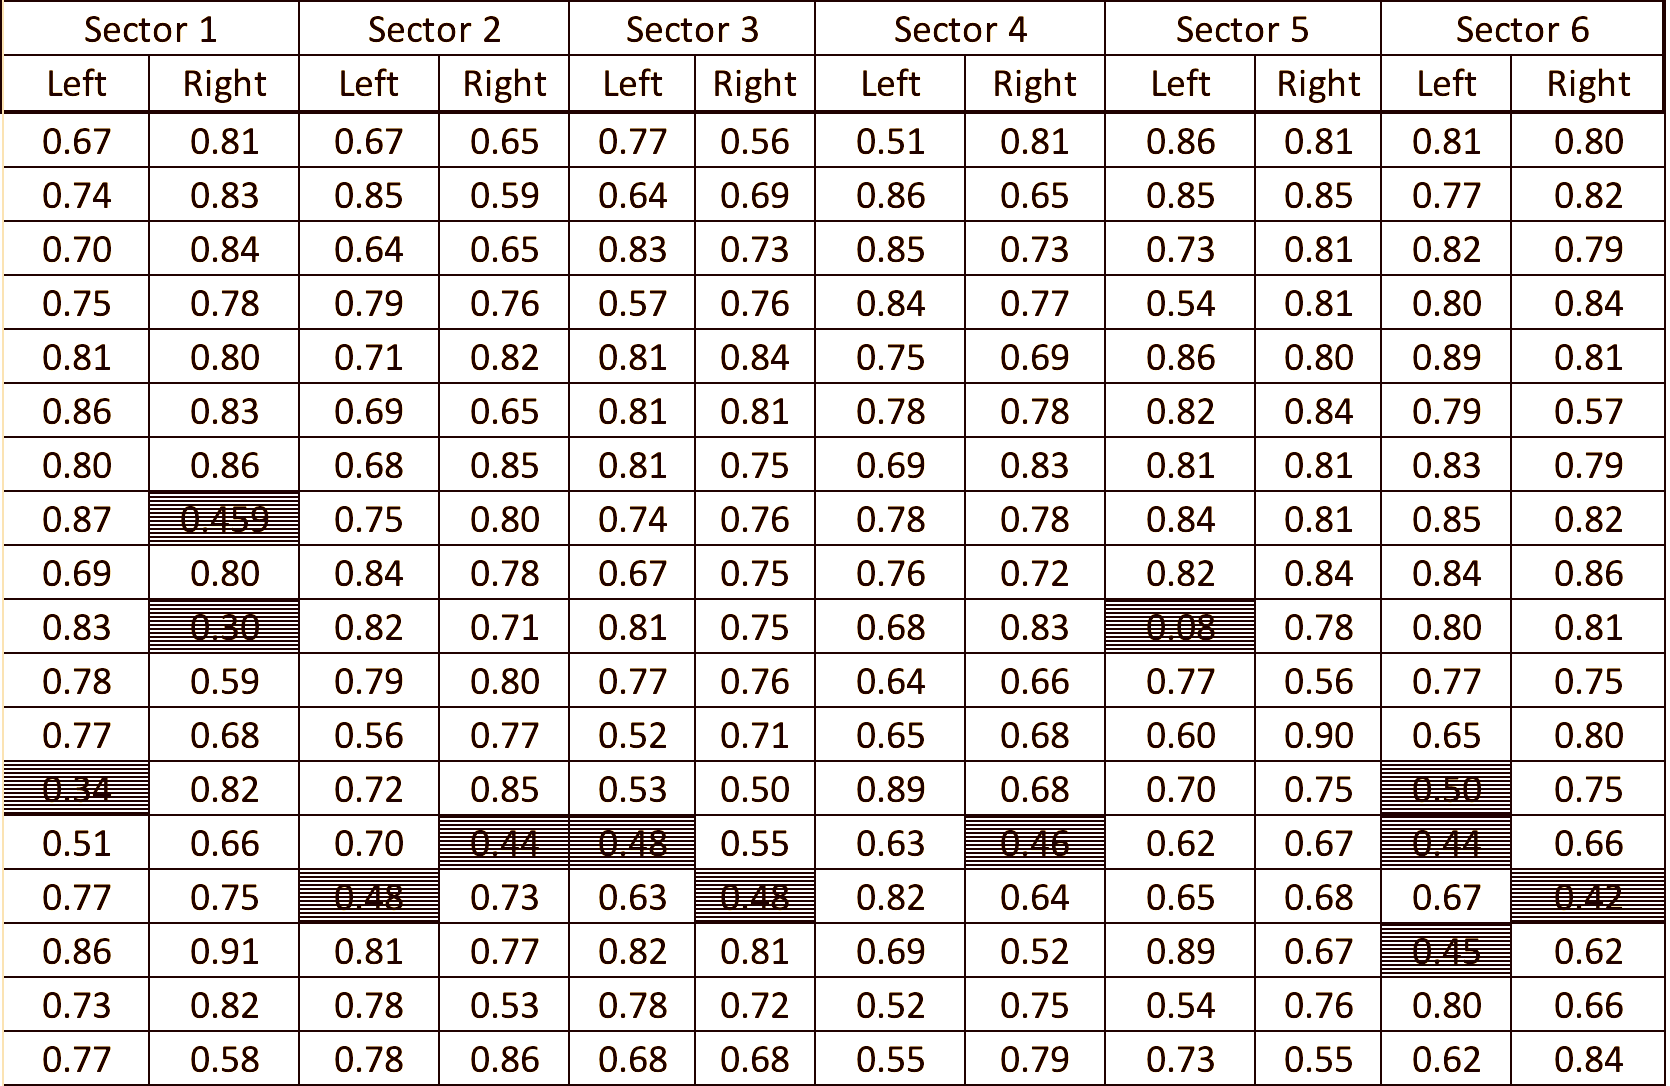
\includegraphics[width=0.95\columnwidth,keepaspectratio]{img/wcStatusAfter.png}
	\caption{Top: typical reflectivity of a ``very poor'' WC after refurbishment.
            The reflectivity quickly rise to $to 65\%$ at a wavelength of about 340 nm. Bottom: average WC reflectivity  $r$ between 200 and 400 nm for
				all the WC. This picture should be compared to \F{wcStatusAfter}. }
	\label{fig:wcStatusAfter}
\end{figure}


